%%%%%%%%%%%%%%%%%%%%%%%%%%%%%%%%%%%%%%%%%%%%%%%%%%%%%%%%%%%%%%%%%%%%%%%%%%%%%%%%%%%%%%
%% Author:      Nils Weber and Maximilian Stiefel
%% Date:        23.12.2017
%% University:  Uppsala Universitet
%% Department:  Institutionen för informationsteknologi 
%% Course:      Embedded Control System Project
%% Project:     PRECISELY CONTROLLED DIY ETCHING MACHINE 
%%				FOR USAGE AT HOME AND IN SMALL LABS
%%%%%%%%%%%%%%%%%%%%%%%%%%%%%%%%%%%%%%%%%%%%%%%%%%%%%%%%%%%%%%%%%%%%%%%%%%%%%%%%%%%%%%

\chapter{Implementation}
\label{chap:implementation}
% Explain explicitly how things have been implemented or are supposed to be implemented i.e. software, hardware, mechanics. 

\section{UV Light}
\label{sec:uv_light}

\begin{figure}[H]                                                         
\centering          
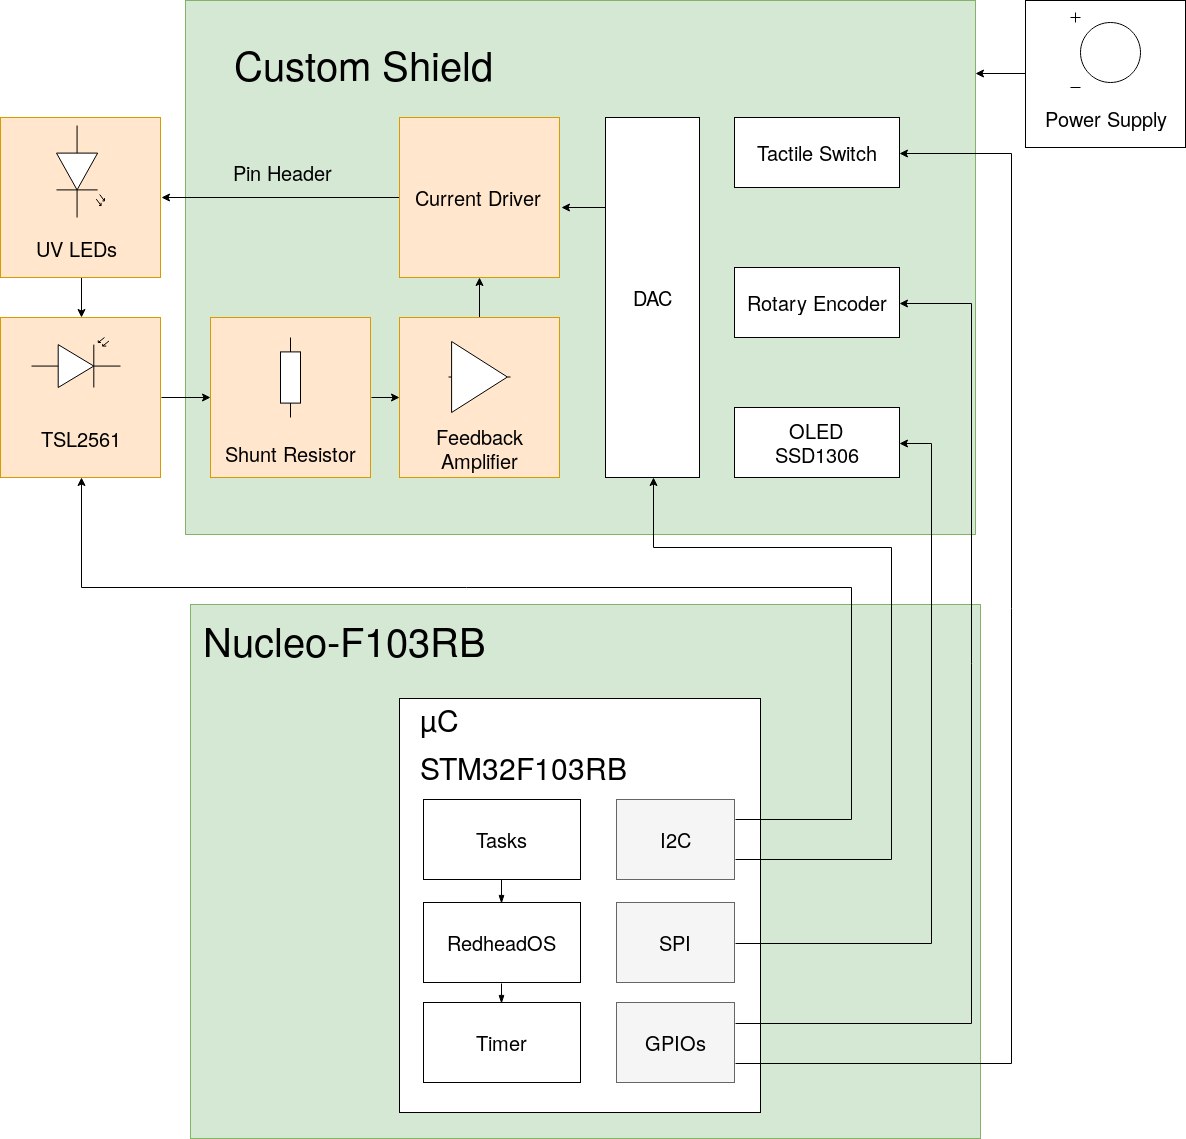
\includegraphics[width=0.8\textwidth]{./fig/uv_light_block_diagram}   
\caption[UV light system.]{UV light system. Top: Custom extension board. Bottom: Nucleo board with custom software.}   
\label{fig:uv_light_block_diagram}                                                       
\end{figure}  

The decision has been made to use the \myemph{Nucleo-F103RB}, a cheap (approx. 25 USD) development board, instead of designing a processor board. This has a couple of advantages:
\begin{itemize}
\item No \gls{PCB} design required to bring the STM32 on a board. 
\item Directly start programming without waiting until the hardware is ready.
\item Debugger and programmer from STM included. 
\item Time to develop something, that works is shortened. 
\end{itemize}
Instead, a custom extension board for the Nucleo board has been designed (cf. fig. \ref{fig:uv_light_block_diagram}). Everything has been laid out so the hardware can drive a lot of \myemph{industry standard T-1 3/4} \SI{5}{\milli\metre} \glspl{LED}. In fact it can supply 256 of these \glspl{LED}. Four \glspl{LED} can be put in series. The voltage drop does not exceed \SI{14}{\volt}. This has been verified by measurements in the lab with a current of \SI{30}{\milli\ampere}. Hence, a power supply of \SI{18}{\volt} is sufficient. Although something closer to \SI{14}{\volt} would be more efficient. However, it does not matter so much, as long as the linear regulator can dissipate enough power without being destroyed. 
\newpar
The \glspl{LED} are meant to be connected with a 64 pin header (low-side) and a 10 pin header to the board. Actually, a rather big housing has been built together to take in the \glspl{LED} and the electronics eventually. 
\newpar 
A small \gls{OS}, developed from scratch, runs on the STM32 to make real-time scheduling possible with a small code footprint and give a programmer all the necessary infrastructure to program conveniently (semaphores, queues, printf etc.). 

\subsection{Hardware}
\label{subsec:uv_light_hw}
\begin{figure}[H]                                                         
\centering          
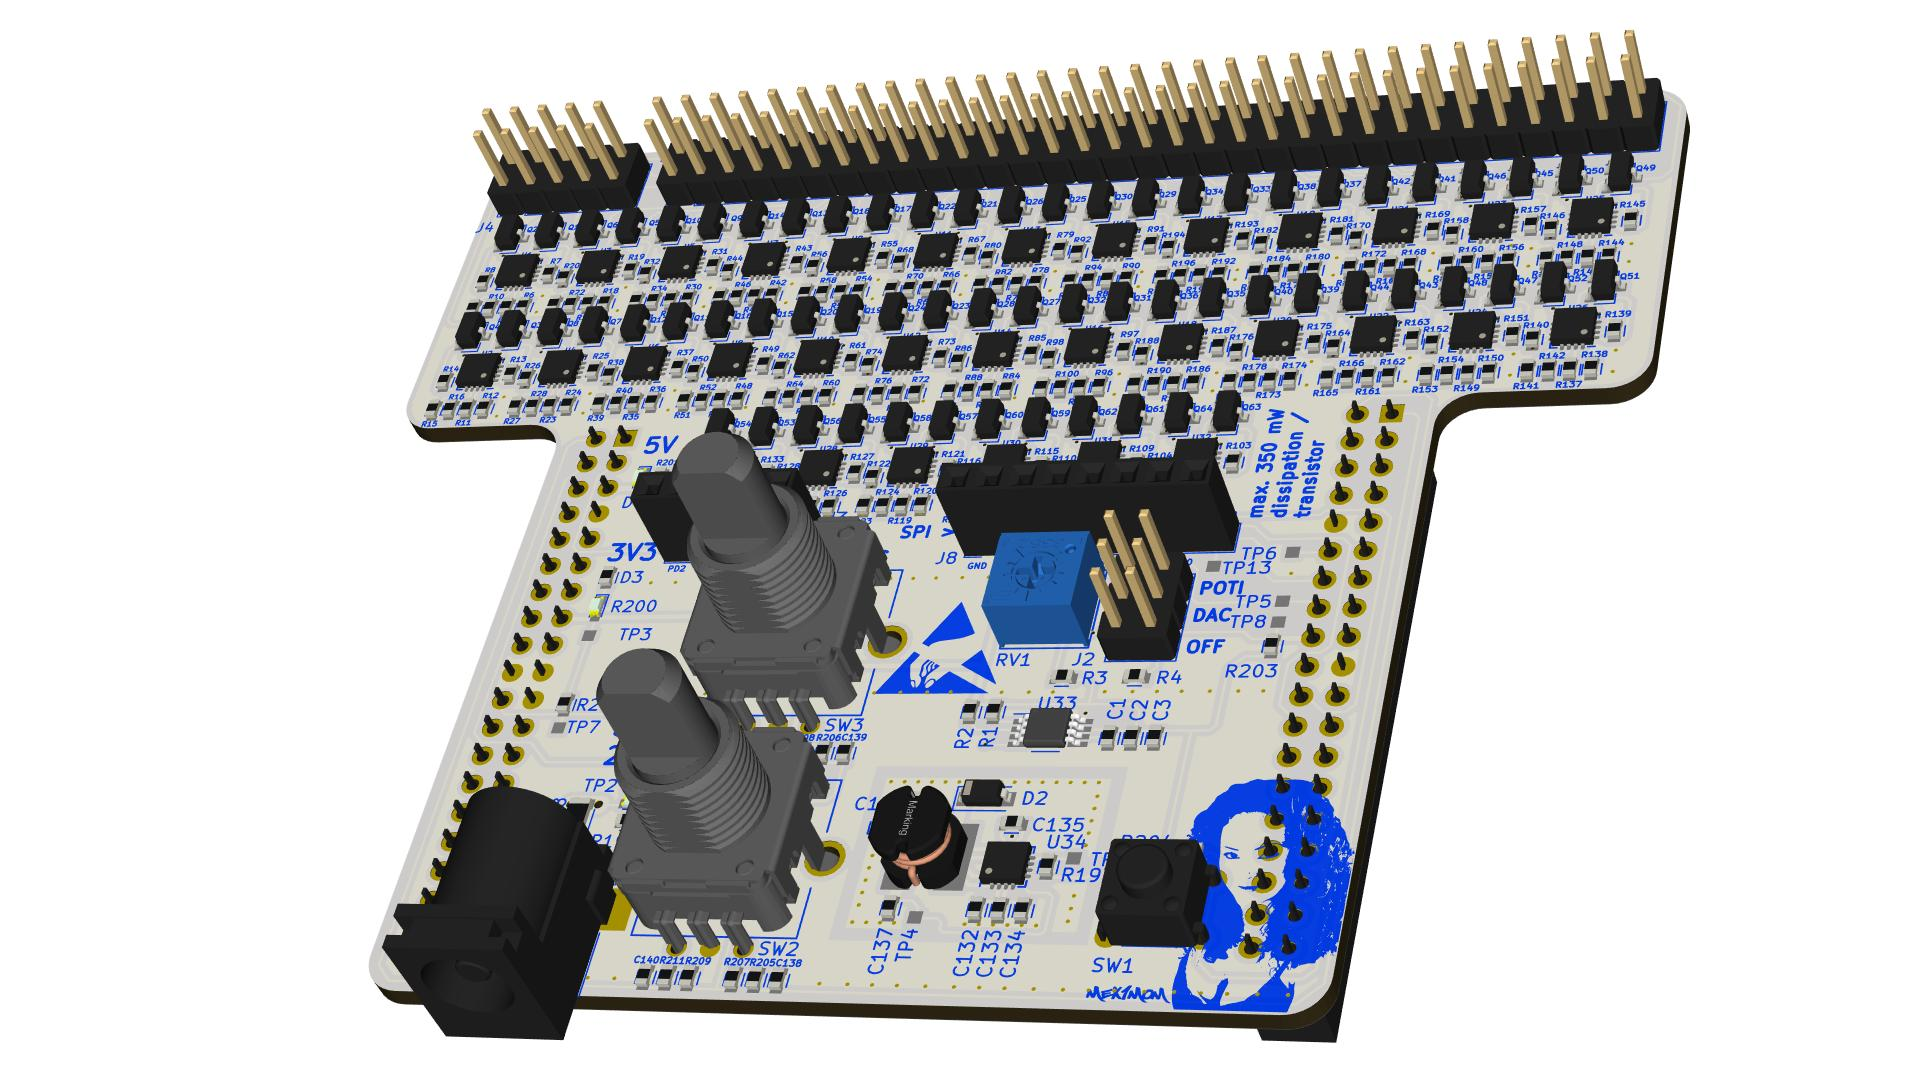
\includegraphics[width=1\textwidth]{./fig/3d_pic_pcb}   
\caption[Four layer extension board for the Nucleo-F103RB.]{Four layer extension board for the Nucleo-F103RB to drive 64 \gls{LED} channels. All 3D models have been entered into the \gls{ECAD} program to prevent unintended surprises.}   
\label{fig:3d_pic_pcb}                                                       
\end{figure}  
The board shown in fig. \ref{fig:3d_pic_pcb} has been developed and produced in the course of this project. It has four layers, but no micro vias, to, on the one hand get a grip on the complexity, and on the other hand save money (micro vias are still expensive than through-hole vias in production, cf. \ref{chap:introduction}). As an introduction, one can briefly list the features of this sophisticated piece of hardware.
\begin{itemize}
\item 64 \gls{LED} driver stages.
\item \SI{6.4}{\ampere} (\SI{0.1}{\ampere} per stage) and \SI{24}{\volt} max. input. 
\item \SI{0.2}{\ampere} max. and \SI{350}{\milli\watt} dissipation max. per stage. Stages can be left floating if unused without the threat of damaging the device. 
\item 10 Bit \gls{DAC} to steer the driver combined with feedback amplification to achieve a tremendously fine resolution. 
\item Optional potentiometer to set the current. 
\item Control loop to guarantee the desired current and respond quickly to changing the setpoint. 
\item 2 rotary encoders and 1 tactile switch.
\item \gls{I2C} header.
\item \gls{SPI} header. 
\end{itemize}

In appendix \ref{append:extension} an extract of the schematics of the board is available. The following lines shall briefly describe the different circuits. One page 1/37 one can see, that there are four main modules: The interface to the processor board, the \gls{LED} driver, the power management and  the user interface. 
\newpar 
On page 2/37 one can see the \gls{LED} driver part. On the right side, the \myemph{DAC101C085} from \myemph{Texas Instruments} is placed. \SI{0}{\ohm} resistors give flexibility in setting the bus address. The reference voltage is connected to the supply voltage of \SI{3.3}{\volt}, provided by the processor board. Below that, one can see a potentiometer and a connector, that can be populated with a jumper to set the reference voltage for the driver accordingly. The reference voltage is translated into a current whereas with the resistor configuration so far \SI{1}{\volt} equals \SI{10}{\milli\ampere}. The last connector on the right side is to make the \gls{I2C} interface 1 of the microcontroller accessible.
On the left side there are 32 times 2 driver stages, which equals a total of 64 driver stages. The group forming is as it is, because the deployed quadruple operational amplifier (\myemph{LM324}) can be used for 2 stages as it has four operational amplifiers inside. In addition, one can see the big 64 pin header for \gls{LED} connection. 
\newpar 
Page 3/37 reveals the \gls{LED} driver design as it shows one driver stage, which consists out of one \myemph{LM324} (four operational amplifiers) and two \myemph{MBT3904} (NPN transistor). The controller works as follows: 
\begin{enumerate}
\item A current \ensuremath{I_C} flows through the transistor into the shunt resistor \ensuremath{R_S}, which is connected to the input of a non-inverting amplifier. 
\item The shunt resistor \ensuremath{R_S} has a small resistance value of \SI{10}{\ohm} and translates the current \ensuremath{I_C} into a voltage \ensuremath{V_S = I_C \cdot R_S}. This might even work with a smaller shunt resistor. 
\item Obviously, the resulting voltage \ensuremath{V_S} is very small, which is why there is an amplifier in the feedback loop. Analyzing this operational amplifier configuration one ends up with the following relation between input and output: 
\begin{equation}
V_{out} = V_{in} \frac{R_1 + R_2}{R_1} = V_{in} \frac{\SI{20}{\kilo\ohm} + \SI{180}{\kilo\ohm}}{\SI{20}{\kilo\ohm}} = 10 V_{in}
\end{equation}
The size of the shunt resistor and the amplification factor determine the mapping between bits set in the \gls{DAC} (10 Bits) and the current through the \gls{LED}. Making the shunt resistor smaller is of course better because of unnecessary heat dissipation, but one has to keep in mind, that the operational amplifier is absolutely low-cost and has a certain offset voltage. Also, the closer one gets to the power supply voltages of the operational amplifier, the more problems of non-linearity occur. 
\item In the last step, the voltage output of the first stage is compared with the setpoint, coming either from the \gls{DAC} or the potentiometer. The output of the second stage is a current \ensuremath{I_B} proportional to the difference between the inputs. 
\begin{equation}
 I_C = I_B \cdot \beta
\end{equation}
is the relation between the base current and the collector current. According to the datasheet \ensuremath{\beta} is somewhere between 100 and 300, which is why a small error is neglected, since \ensuremath{I_C \gg I_B}: The current into the transistor collector is not the same as the current going out of the emitter. Hence, the current through the \glspl{LED} is about less then 1 \% smaller than the current the controller is aware of. 
\end{enumerate} 
The power distribution becomes clear taking a look at page 35/37. Using a barrel jack a lot of standard power supplies can be interfaced with the board. The board design is \myemph{IPC 2221} compliant given the parameters one can see in the schematics. A powerful buck converter \gls{IC} the \myemph{TS30011} steps down the input voltage to \SI{5}{\volt}. The processor board can be powered with external \SI{5}{\volt}, assumed that configured correctly. \SI{3.3}{\volt} can then be obtained from the processor board to supply e.g. the \gls{DAC} or the \gls{OLED} screen on the extension board. 
\newpar 
Page 36/37 shows the interfacing between processor and extension board. Nothing to really see here. 
\newpar 
The small user interface is on the last page 37/37. One connector enables access to the \gls{SPI} 1 of the microcontroller. Also one finds the tactile switch and two rotary encoders, which are debounced hardware wise. 

\subsection{Software}
\label{subsec:uv_light_sw}

\begin{figure}[H]                                                         
\centering          
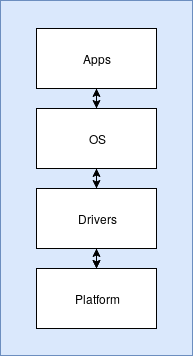
\includegraphics[width=0.3\textwidth]{./fig/layering}   
\caption[Layered code structure]{Layered code structure}   
\label{fig:layering}                                                       
\end{figure}

Fig. \ref{fig:layering} shows how the code ought to be structured in general. This allows to migrate the actual functionality quickly to another platform. However, as it turned out it can be hard sometimes not run into layer breaches i.e. the code one layer is supposed to only communicate with the layer above and the layer below if implemented properly.  
\newpar 
Every kind of controller is implemented in the \myemph{App layer}. The \gls{OS} layer provides a \gls{PID} controller infrastructure. A task is running, which handles the controller for the \gls{UV} light intensity, that gets the feedback input from the light sensor and steers the \gls{DAC}.
\newpar 
The \gls{DAC} driver is implemented in the \myemph{Driver layer}, whereas this driver needs to use \gls{I2C}, which is a hardware component of the \myemph{STM32}. \gls{I2C} is for this reason located in the \myemph{Platform layer}. Switching to another microcontroller, one ideally only needs to change the \myemph{Platform layer}. 
\newpar 
The \gls{OLED} screen driver belongs into the \myemph{Driver layer} accordingly and there are tasks to handle the user input from the rotary encoders and the switch in the \myemph{App layer}.  

\subsection{Mechanics}
\label{subsec:uv_light_mechanics}

\begin{figure}[H]                                                         
\centering          
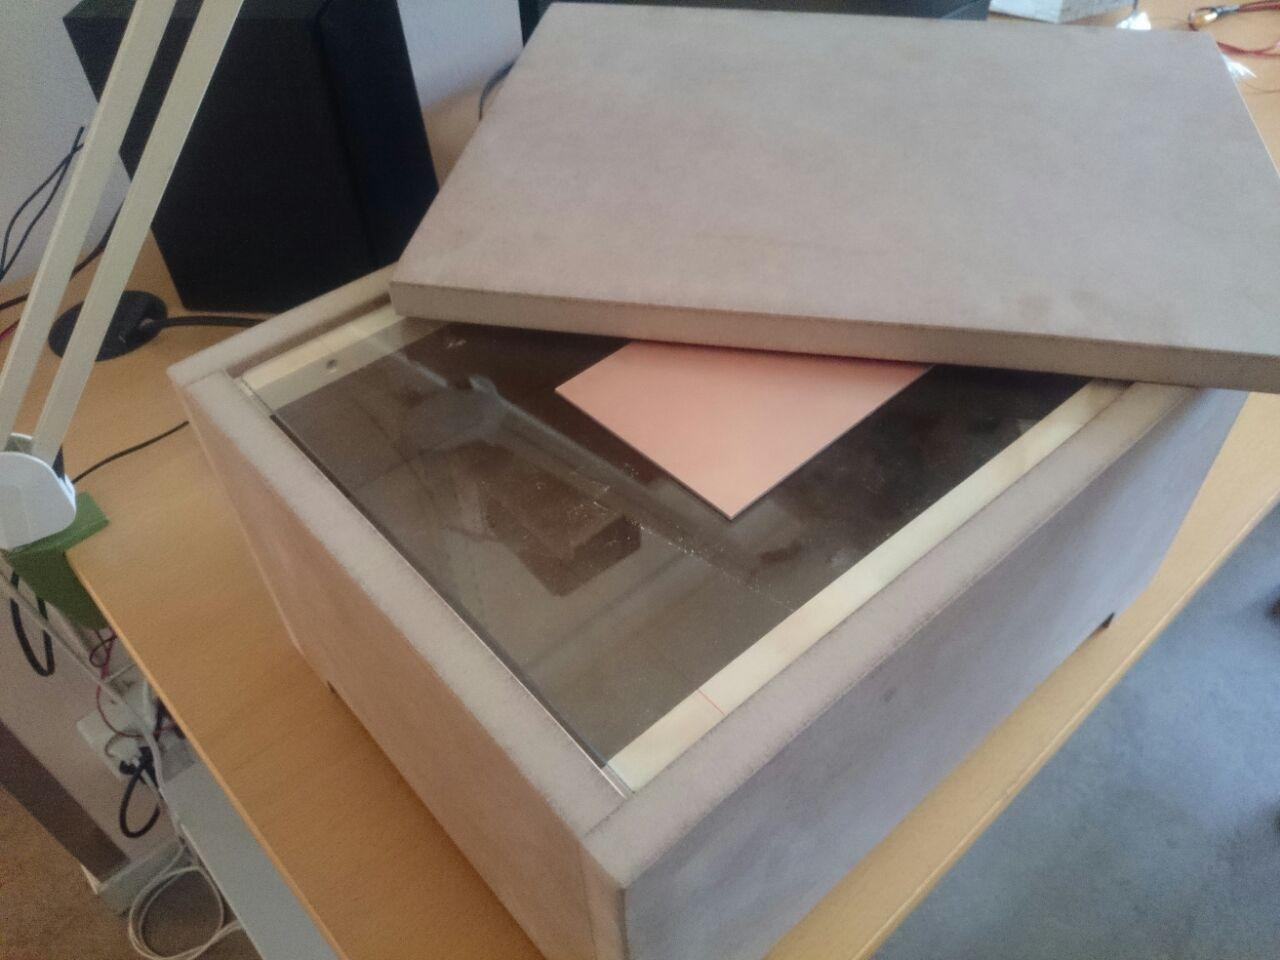
\includegraphics[width=0.6\textwidth]{./fig/uv_lamp_box}   
\caption[Wooden box for the \gls{UV} exposer unit.]{Wooden box for the \gls{UV} exposer unit with 16 x 16 \gls{LED} matrix.}   
\label{fig:uv_lamp_box}                                                       
\end{figure} 

In cooperation with a carpenter a wooden box has been build, which uses a glass plate from an old scanner (cf. fig. \ref{fig:uv_lamp_box}). A wooden plate is located below the glass. On this wood plate there is a matrix out of 256 \glspl{LED}. The distance between glass and \gls{LED} matrix can be varied with the help of IKEA parts, that are plugged into the sidewalls while simultaneously holding the \gls{LED} matrix. The cabling, drilling and soldering to create the \gls{LED} matrix is a nightmare as one can imagine. Each single \gls{LED} needs to be connected to wires to lengthen the legs of it. Subsequently, every \gls{LED} is fixed in a hole and fixed with a hot glue gun. Always four \glspl{LED} have to be connected together in series. Eventually, every single one of the 64 stages has to be connected somehow to the extension board. For this reason a small adapter \gls{PCB} has been constructed (cf. fig. \ref{fig:adapter_board}). This board can be installed with wood screws and high- and low-side of the \glspl{LED} can be soldered. Following, one just has to plug in the two ribbon cables.   

\begin{figure}[H]                                                         
\centering          
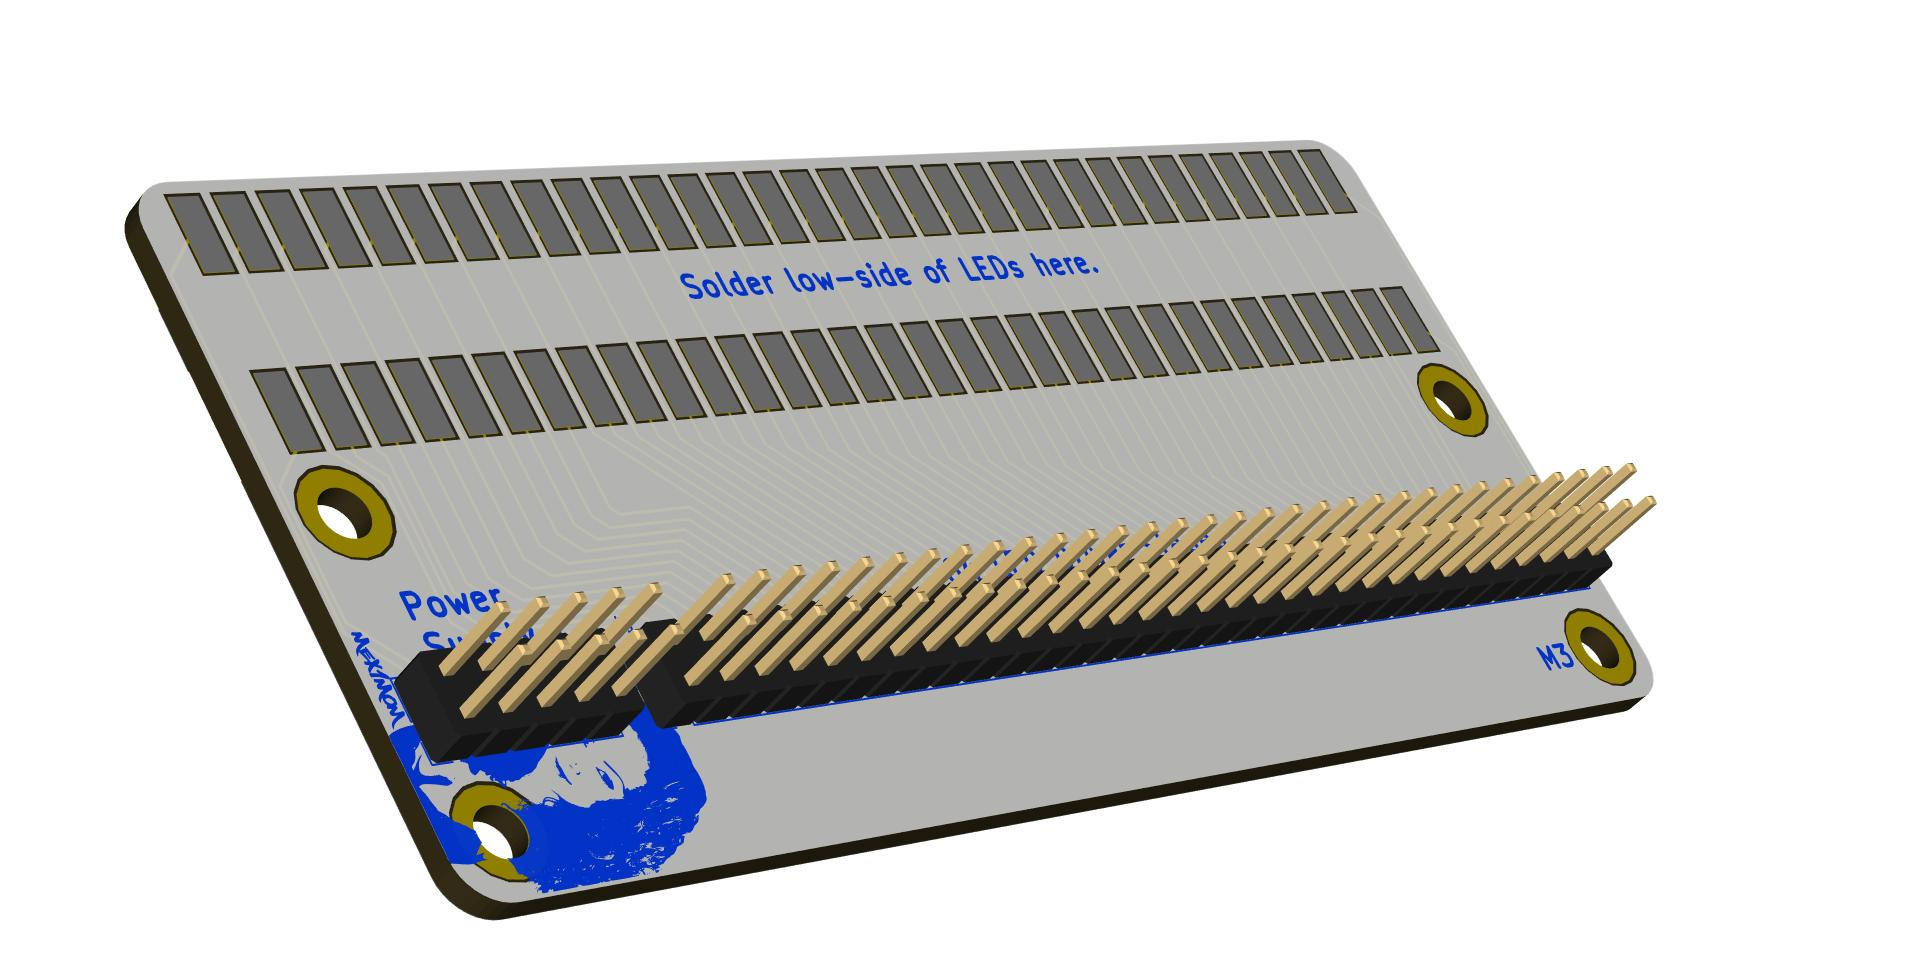
\includegraphics[width=0.8\textwidth]{./fig/3d_pic_2}   
\caption[Adapter board for \gls{LED} matrix enables simple plug and play.]{Adapter board for \gls{LED} matrix enables simple plug and play after soldering high- and low-side of the \gls{LED} strings.}   
\label{fig:adapter_board}                                                       
\end{figure} 


\section{Etching Tank}
\label{sec:etching_tank}
As briefly outlined in section \ref{sec:uv_light}, the Nucleo-F103RB has been chosen. During the development of the temperature control the Nucleo-L073RZ has been used for the simple reason of immediate availability. This led to more complications that originally anticipated, as discussed later in chapter \ref{chap:evaluation}.

\subsection{Hardware}
\label{subsec:etching_tank_hw}
Less sophisticated is the electric hardware for the temperature control, as it is in early prototyping stage to date and future tests will provide knowledge to chose the smartest path in further developments.
As shown earlier in fig. \ref{fig:etching_bath_simple} the system output is a 50W heater which is controlled via a relay. Its power source is a common power outlet of 230VAC. This relay is optocoupled to a normal digital output GPIO for security reasons.
For the user interface a small OLED screen with the SSD1306 driver and I2C interface is used as output, and a rotary encoder is used as input. The screen shows the temperature inside the etching bath, the reference temperature and the ambient temperature.
Since no cooling mechanism is installed, the reference temperature cannot be set below the ambient temperature.

\subsection{Software}
\label{subsec:etching_tank_sw}
Core of the system is the control algorithm implemented as described in \cite{article:onoffPLC}. The algorithm shown in fig. \ref{fig:inertiaCorrectionProp} has been implemented in \myemph{c} and is briefly described in the following. The names of the variables are chosen 
according to \cite{article:onoffPLC}.

A simple on-off controller is of course the heart of the algorithm. It determines a binary output based upon the corrected control error \(V\) and the hysteresis \(H\).

\begin{minted}[baselinestretch=1, fontsize=\small, linenos,frame=single,framesep=5pt]{C}
uint8_t onOffController(double iV, double iH) {
  uint8_t oU = 0;

  if (iV >= (iH/2)) {
    oU = 1;
  }
  else if (iV <= (iH/2)) {
    oU = 0;
  }

  return oU;
}
\end{minted}

The above described on-off controller is embedded in the following function, which would be called from the main program or called in a periodic task.
At first, the input parameters are re-scaled using the function \texttt{u\_map()} shown further below. The negative feedback is re-scaled to a ranged from 0 to 1, while the reference value is scaled to 0 to 100.
After the re-scaling the algorithm computes the proportional correction and calculates the control error based upon that value.
Next, the inertia correction is applied to the current value using the inertia correction value from the previous computation.
Now the on-off controller is called with the modified values from proportional and inertia corrections.
As a last step before returning the binary output value, the next inertia correction value is computed calling the respective function described below.

\begin{minted}[baselinestretch=1, fontsize=\small, linenos,frame=single,framesep=5pt]{C}
uint8_t controller(uint8_t _nowT, uint8_t _aimT) {
  double deltaT = 1; // HAS TO BE DETERMINED!!
  double K_k = 10.0;
  double T_k = 0.01;
  double H = 1; // HAS TO BE DETERMINED!!

  double A = (deltaT*K_k)/T_k;
  double B = 1-(deltaT/T_k);

  static double nW; // keep inertia correction value


  // re-scale input parameters
  double nY = ((double) u_map(_nowT, 0, 100, 0, 100))/100;
  double nR = (double) u_map(_aimT, 0, 100, 0, 100);

  // proportional correction
  double nP = nR * (1+K_k); // C = 1 + K_k

  // calculate error
  double nE = nP - nY;

  // apply inertia correction
  double nV = nE - nW;

  // call on-off controller
  uint8_t bU = onOffController(nV, H);

  // call inertia correction
  nW = inertiaCorrection(bU, nW, A, B);

  return bU;
}
\end{minted}

Following equation is implemented in the inertia correction function.
\begin{equation}
W_{t(i)} = AU_{t(i-1)}+BW_{t(i-1)}
\end{equation}
where
\begin{align}
A&=\frac{\Delta t K_k}{T_k} \\
B&=1-\frac{\Delta t}{T_k}
\end{align}

\begin{minted}[baselinestretch=1, fontsize=\small, linenos,frame=single,framesep=5pt]{C}
double inertiaCorrection(uint8_t fU, double nW, double A, double B) {
  double UA, WB;
  UA = ((double)fU)*A;
  WB = nW*B;

  return (UA+WB); //nW
}
\end{minted}

\begin{minted}[baselinestretch=1, fontsize=\small, linenos,frame=single,framesep=5pt]{C}
uint32_t u_map(uint32_t x, uint32_t in_min, uint32_t in_max, 
			   uint32_t out_min, uint32_t out_max) {
  return (x - in_min) * (out_max - out_min) / (in_max - in_min) + out_min; 
  }
\end{minted}

Other than that, the rotary encoder is implemented to easily adjust the wanted temperature. Both, the realtime and wanted temperature are shown on the display via I2C.

\subsection{Mechanics}
\label{subsec:etching_tank_mechanics}

The etching tank has been produced of a mix of glass and additive manufactured plastic parts to add functionality and form.
The lid and floor are shown in fig. \ref{fig:lidFloor}. Between lid and floor is a tank made of glass, seen in fig. \ref{fig:tank}. Inside this tank, hanging from the lid, is a U-shaped system to hold the PCB. Its size is adjustable to the PCB and maximum 148 mm x 160 mm. The technical drawings are attached in appendix \ref{append:techDrawPCB}. On the right side one can also see the heater and in the bottom a thinner black tube. This tube is connected to a compressor and ejects the air bubbles to speed up the removal of copper from the PCB.

\begin{figure}[H]
\centering          
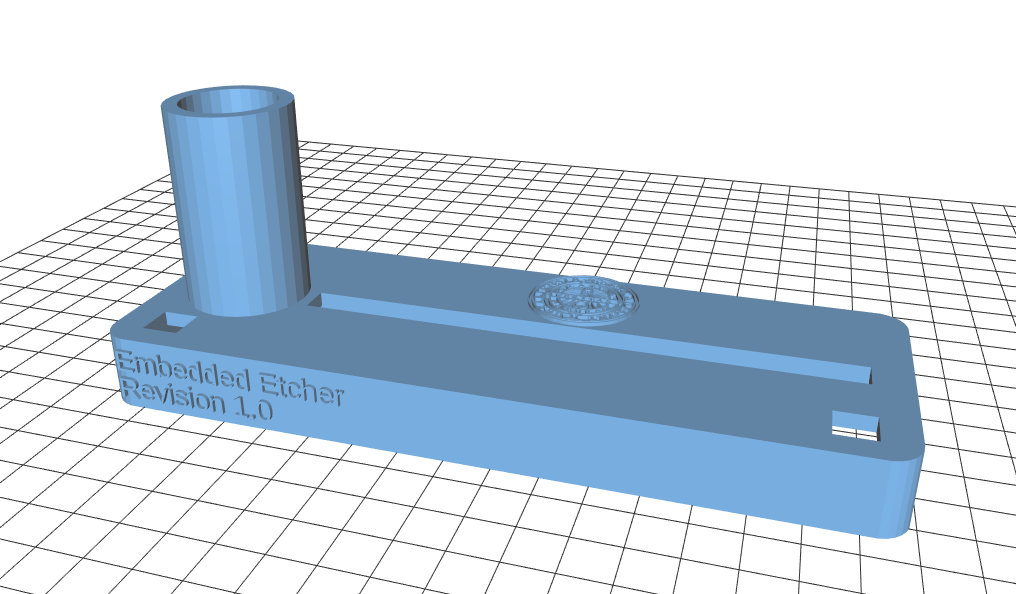
\includegraphics[width=0.6\textwidth]{./fig/lid}   
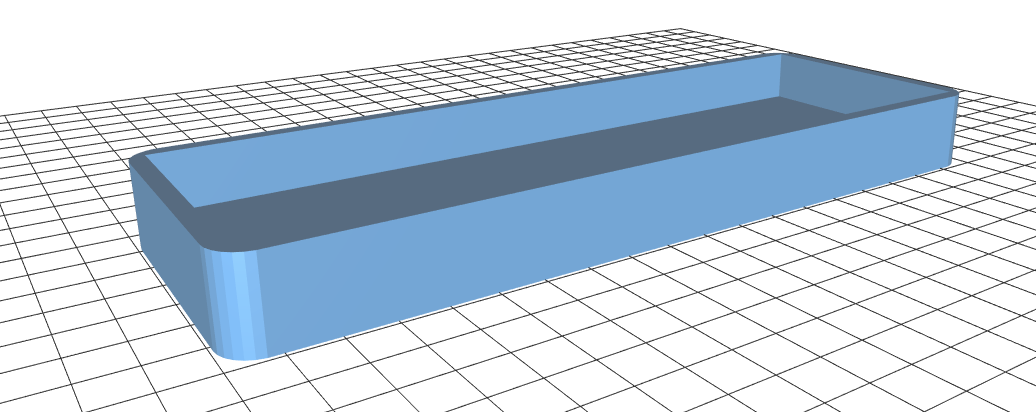
\includegraphics[width=0.6\textwidth]{./fig/floor} 
\caption[Lid and floor of the etching tank.]{Lid and floor of the etching tank.}   
\label{fig:lidFloor} 
\end{figure}

% \begin{figure}[H]
% \centering  
% 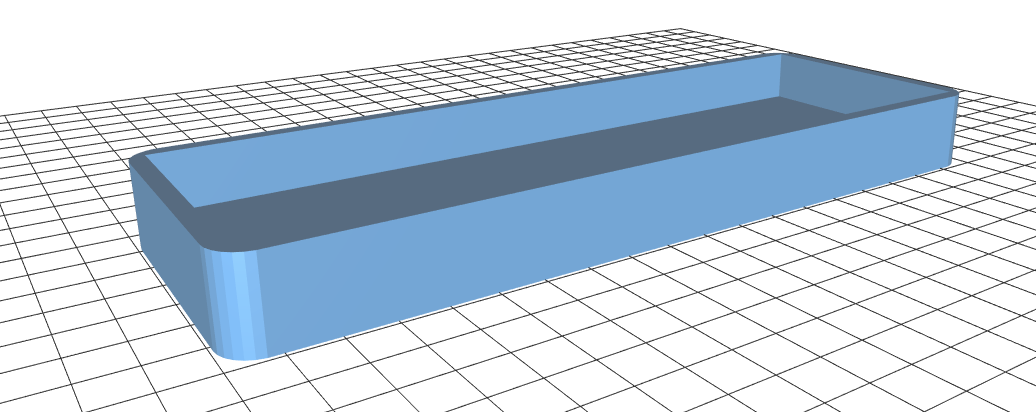
\includegraphics[width=0.6\textwidth]{./fig/floor}   
% \caption[Floor of the etching tank.]{Floor of the etching tank.}   
% \label{fig:floor} 
% \end{figure} 

\begin{figure}[H]
\centering  
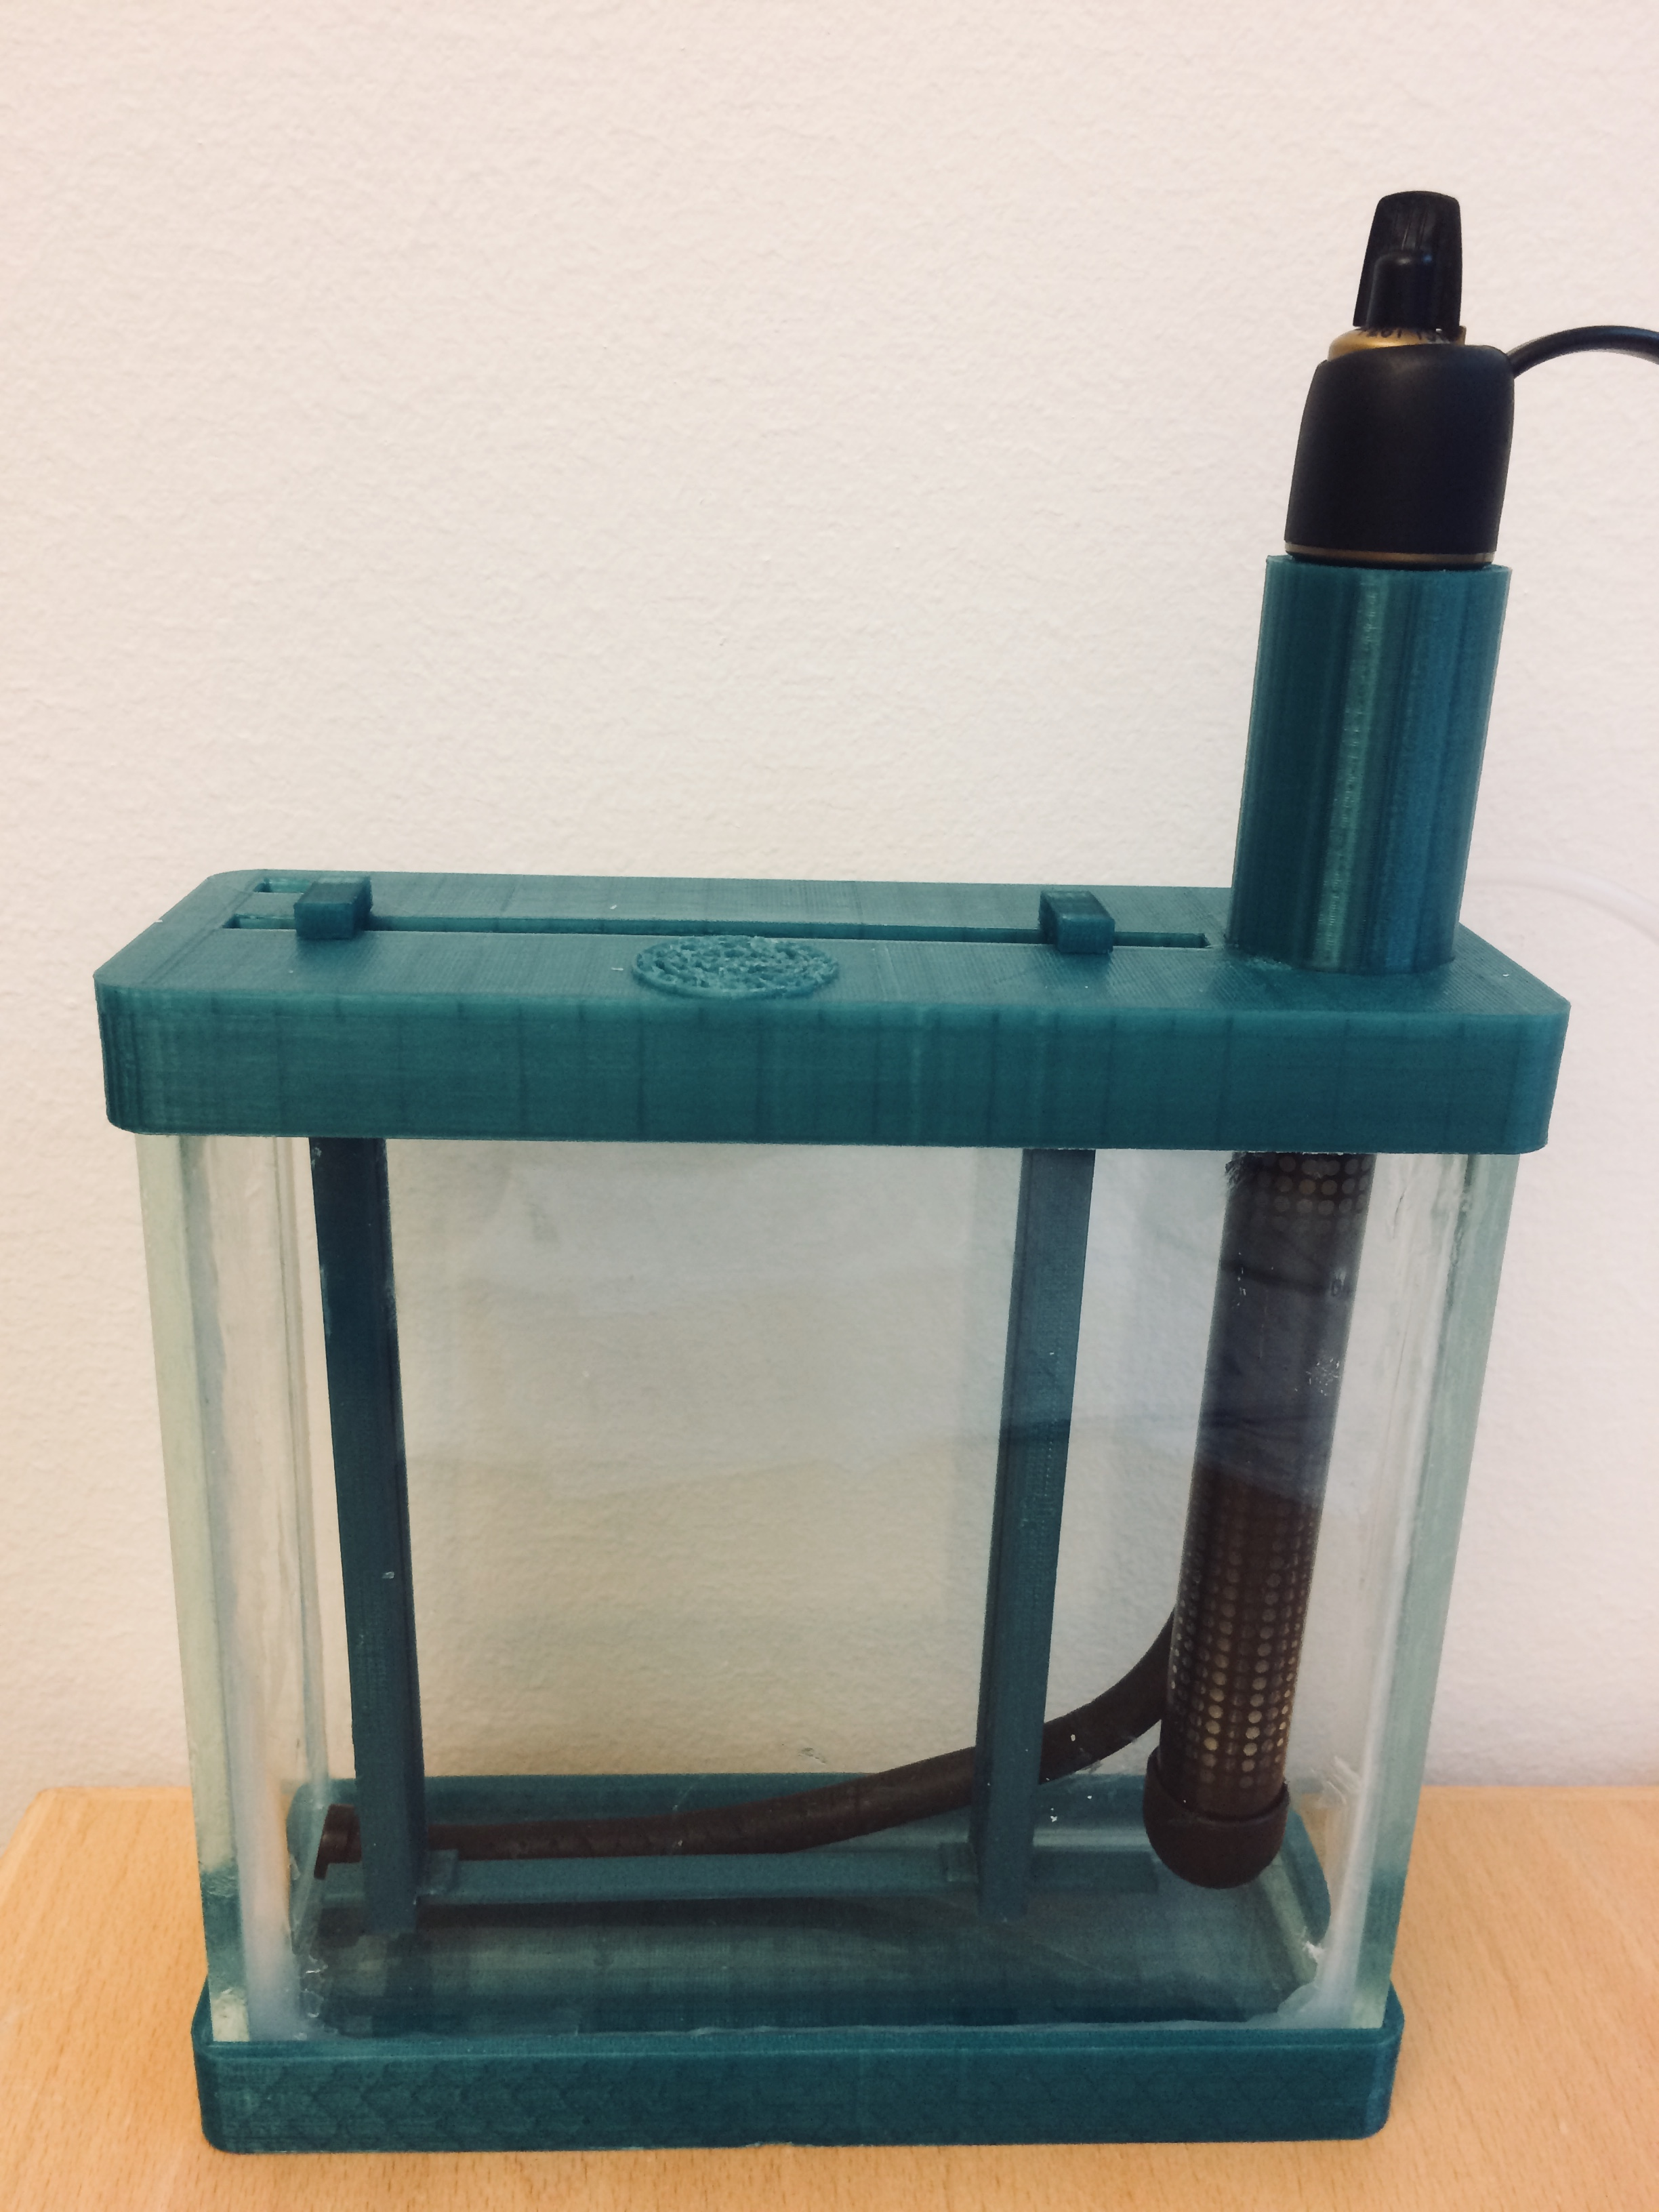
\includegraphics[width=0.6\textwidth]{./fig/tank}   
\caption[The etching tank.]{The etching tank.}   
\label{fig:tank} 
\end{figure}

\section{Operating System}
\label{sec:os}

\begin{figure}[H]                                                         
\centering          
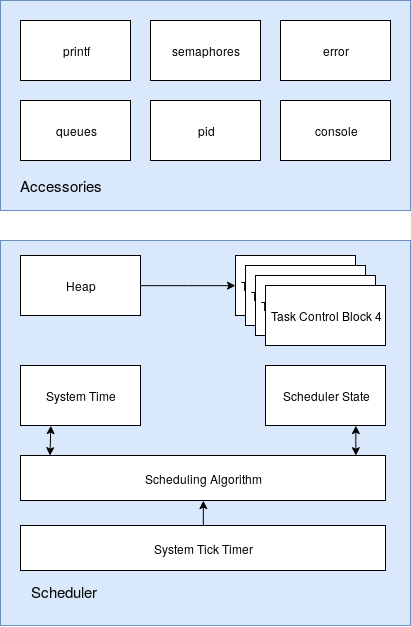
\includegraphics[width=0.5\textwidth]{./fig/redhead_os}   
\caption[Structure of the \gls{OS}]{Structure of the \gls{OS}}   
\label{fig:redhead_os}                                                       
\end{figure}  

In the course of the project a small real-time \gls{OS} has been developed. Fig. \ref{fig:redhead_os} shows how the \gls{OS} is structured. The operating system kernel consists out of a pretty simple scheduler, which is hooked up to the system tick timer, that the \myemph{Cortex-M3} (in the case of the \myemph{STM32F103RB}) provides. Configuring the system tick period is possible. With every system tick the scheduling algorithm is invoked. A state machine is deciding how to handle the system tick. Moreover, the scheduling is based on a binary heap, that contains pointers to the \glspl{TCB} of the tasks, which are supposed to be executed. A task control block is created, when a task is spawned by a programmer with. This works as follows:

\begin{minted}[baselinestretch=1, fontsize=\small, linenos,frame=single,framesep=5pt]{C}
/** Spawn a task.
 *
 * @param ifnc_ptr Pointer to the task function.
 * @param itask_name Internal task name.
 * @param iarguments Enables passing user-defined arguments to the task.
 * @param ipriority A higher value means a higher priority of the task.
 * @param oTaskHandle Pointer to TCB.
 * @retval 1 (task has been spawned) or 0 (FAILED)
 */
uint8_t osTaskCreate(void (*ifnc_ptr)(void*), char* itask_name, void* iarguments, 
	uint8_t ipriority, const osTCB_t* oTaskHandle);
\end{minted}

In general the \gls{OS} interface is frankly speaking inspired by FreeRTOS\texttrademark{}. One can also see, that the scheduling is priority based. The task with the highest priority is always executed as soon as the current task finished its job. Priorities can not be changed on run-time. Of course, as with any real-time \gls{OS} delay functions are available. \myemph{osTaskDelayUntil} is the more important one, as it allows periodic task execution. 

\begin{minted}[baselinestretch=1, fontsize=\small, linenos,frame=single,framesep=5pt]{C}
void task3(void* ptr)
{
	static uint32_t wakeup = 0;
	char* args = (char*)ptr;

	wakeup = osSchedulerGetSysT();
	DEBUG_MSG("%s here!\n\r", args);
	osTaskDelayUntil(wakeup, MS_2_TICKS(300));
}
\end{minted}

As shown in the example above the \gls{TCB} also holds a pointer to data, that can be passed to a task. 
\newpar 
Besides creating a easily understandable real-time \gls{OS} it was intended to provide some smooth infrastructure with it, or rather to equip it with some tools, so that one does not always have to reinvent the wheel, kicking off a new project. Therefore, the \gls{OS} comes with a growing set of accessories as for instance queues (cf. accessories in fig. \ref{fig:redhead_os}). 

\begin{minted}[baselinestretch=1, fontsize=\small, linenos,frame=single,framesep=5pt]{C}
void USART2_IRQHandler(void)
{
	/* USART2 receive buffer contains a char. */
	if(USART_GetITStatus(USART2, USART_IT_RXNE) == SET)
	{
		uint8_t data;
		data = USART_ReceiveData(USART2) & 0xFF;
		if(!osEnqueue(&usart_rx_q, (void*)&data))
			THROW_ERROR(E_USART_RX_BUFFER_OVERLOW);
	}

	/* USART2 transmit buffer empty. */
	if(USART_GetITStatus(USART2, USART_IT_TXE) == SET)
	{
		uint8_t data;
		if(osDequeue(&usart_tx_q, &data))
			USART_SendData(USART2, data);
		else
		{
			/* Nothing to send. Disable interrupt. */
			USART_ITConfig(USART2, USART_IT_TXE, DISABLE);
			tx_overflow = 0;
		}
	}
}
\end{minted}
The code example above shows how the error and the queue accessories can be used to implement the \gls{USART} \gls{IRQ} handler of the \myemph{STM32F103RB} elegantly. The \gls{USART} status register has to be checked for finding out which event triggered the interrupt. Either the transmit buffer is empty again and needs to be fed or the receive buffer contains a char, which needs to be stored somewhere. Both buffers are only as big as 8 bit, so one needs queues, that can be emptied and filled by concurrent processes. The \gls{OS} takes care of that. Also, in this example one can see how an error is passed to the according module in case, the receive buffer overflows. The idea is to have a proper log of what is going on in case the system fails (where did it go wrong and when). Also the sink for error logging can be changed (\gls{EEPROM} / \gls{USART} / screen).
\newpar 
Other accessories are 
\begin{itemize}
\item printf - A light version of \gls{GNU} printf. 
\item semaphores - Different kind of semaphores to get rid of data inconsistency problems that occur with concurrent processes e.g. tasks. 
\item pid - Infrastructure for \gls{PID} controll. 
\item console - A console to command the system and get feedback, similar to a terminal. 
\end{itemize}

The whole \myemph{Doxygen} documentation can be found on \myemph{Github}. 


% \section{Rotary encoder}
% The rotary encoder used for testing and development has a theoretically simple output, however it is of a rather bouncy and thus bad quality, as shown in figure~\ref{fig:re}. Depending on the turning direction either channel A or channel B gets low first and the first one gets high again while the second is still low.
% \begin{figure}[H]
% 	\centering
% 	\includegraphics[width=.8\linewidth]{./fig/re.jpg}
%     \label{fig:re}
% \end{figure}
% Due to many bounces, working with flags, similar to semaphores, is a good option to simply ignore all the bounces. However, one is then restricted to the frequency of calling \texttt{main()}.



